\documentclass[../capitulos/cap1.tex]{subfiles}

\tikzset{every picture/.style={line width=0.75pt}} %set default line width to 0.75pt

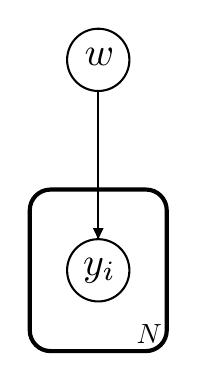
\begin{tikzpicture}[x=0.75pt,y=0.75pt,yscale=-0.6,xscale=0.6]
%uncomment if require: \path (0,300); %set diagram left start at 0, and has height of 300

\draw    (316, 50) circle [x radius= 25, y radius= 25]  ;
\draw    (316, 219) circle [x radius= 25, y radius= 25]  ;
\draw    (316,75) -- (316,194) ;
\draw [shift={(316,194)}, rotate = 270] [fill={rgb, 255:red, 0; green, 0; blue, 0 }  ] [draw opacity=0] (8.93,-4.29) -- (0,0) -- (8.93,4.29) -- (8.93,-4.29)    ;

\draw  [line width=1.5]  [rounded corners= 7.5] (261, 154.14) rectangle (371, 283.86)   ;

\draw (317,48) node [scale=1.44]  {$\boldsymbol{w}$};
\draw (317,219) node [scale=1.44]  {$y_{i}$};
\draw (357,270) node   {$N$};


\end{tikzpicture}
